\section{Sơ đồ Class Diagram}


\begin{figure}[H]
    \centering
    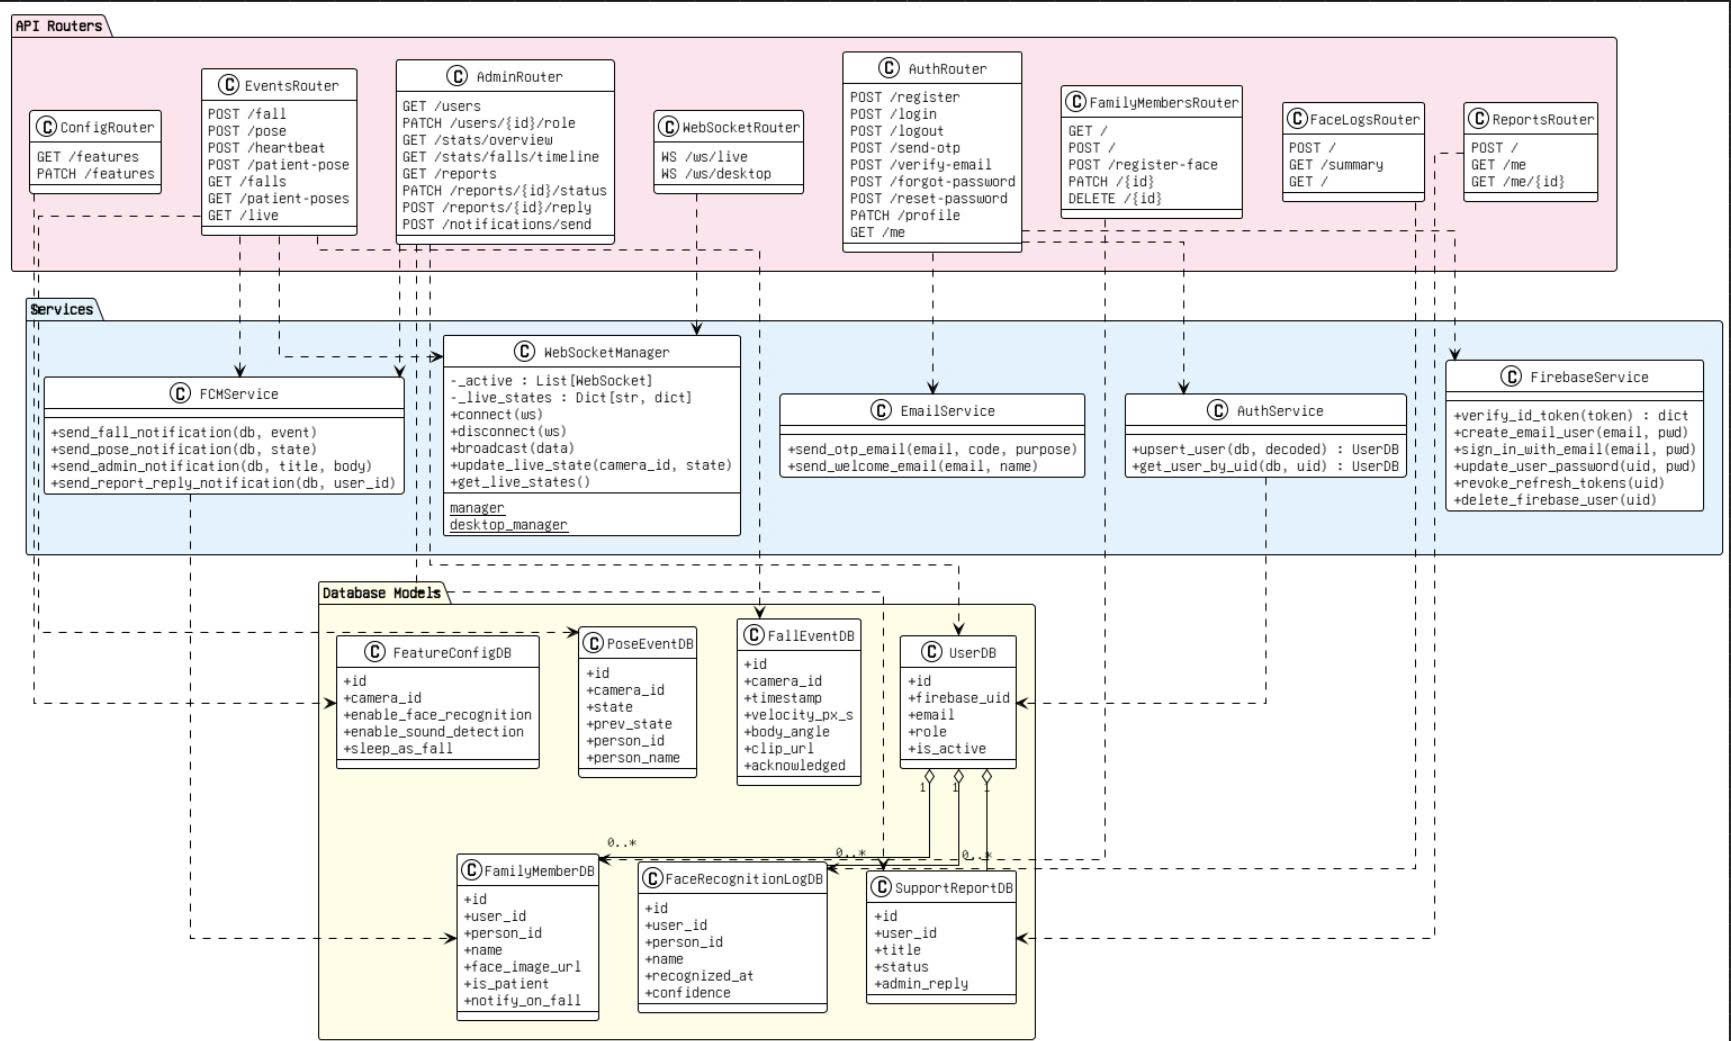
\includegraphics[width=1.0\textwidth]{figures/class_diagram.jpg}
    \caption{Sơ đồ Class Diagram}
    \label{fig:class_diagram}
\end{figure}

\subsection*{Mô tả Class Diagram}

Class diagram của hệ thống được xây dựng theo kiến trúc phân tầng, gồm ba nhóm thành phần chính: \textbf{Database Models}, \textbf{Services} và \textbf{API Routers}. Cách tổ chức này giúp phân tách rõ ràng giữa tầng lưu trữ dữ liệu, tầng xử lý nghiệp vụ và tầng giao tiếp API, từ đó tăng khả năng mở rộng, bảo trì và tái sử dụng mã nguồn.

\subsubsection*{Database Models}

Nhóm này bao gồm bảy lớp thực thể ánh xạ trực tiếp với các bảng trong cơ sở dữ liệu, chịu trách nhiệm lưu trữ và quản lý dữ liệu của hệ thống.

\begin{itemize}
\item UserDB: Lưu trữ thông tin tài khoản người dùng như \textit{firebase\_uid}, email và vai trò hệ thống. Đây là lớp trung tâm của hệ thống, có quan hệ một-nhiều với các lớp FamilyMemberDB, FaceRecognitionLogDB và SupportReportDB nhằm quản lý dữ liệu liên quan đến từng người dùng.

\item FallEventDB: Đại diện cho các sự kiện té ngã được phát hiện từ camera giám sát. Lớp này lưu các thông tin như thời điểm xảy ra, vận tốc di chuyển theo pixel, góc cơ thể, đường dẫn video clip và trạng thái xác nhận sự kiện.

\item PoseEventDB: Lưu trữ các sự kiện liên quan đến tư thế bất thường của đối tượng được giám sát. Ngoài trạng thái hiện tại và trạng thái trước đó, lớp còn ghi nhận thông tin nhận diện như định danh và tên người được phát hiện.

\item FamilyMemberDB: Quản lý danh sách người thân được đăng ký trong hệ thống. Thực thể này lưu thông tin khuôn mặt, trạng thái bệnh nhân và tuỳ chọn nhận thông báo khi xảy ra té ngã hoặc sự cố.

\item FaceRecognitionLogDB: Ghi nhận lịch sử nhận diện khuôn mặt, bao gồm tên đối tượng, thời gian nhận diện và độ tin cậy của mô hình AI trong từng lần nhận diện.

\item SupportReportDB: Lưu trữ các báo cáo hỗ trợ hoặc phản hồi từ người dùng. Ngoài nội dung báo cáo, lớp còn quản lý trạng thái xử lý và phản hồi từ quản trị viên.

\item FeatureConfigDB: Quản lý cấu hình tính năng cho từng camera giám sát, bao gồm các tuỳ chọn như nhận diện khuôn mặt, phát hiện âm thanh bất thường và chế độ xem trạng thái ngủ như té ngã.

\end{itemize}

\subsubsection*{Services}

Nhóm Services chịu trách nhiệm xử lý logic nghiệp vụ và đóng vai trò trung gian giữa tầng API và tầng dữ liệu.

\begin{itemize}
\item WebSocketManager: Quản lý các kết nối WebSocket theo thời gian thực giữa desktop và mobile. Lớp duy trì hai instance tĩnh cho từng loại thiết bị, hỗ trợ phát sóng dữ liệu trực tiếp và theo dõi trạng thái hoạt động của camera.

\item AuthService: Xử lý các nghiệp vụ xác thực và đồng bộ tài khoản người dùng. Lớp thực hiện cơ chế \textit{upsert} dữ liệu người dùng vào cơ sở dữ liệu dựa trên thông tin token đã được xác minh.

\item FirebaseService: Đóng vai trò giao tiếp với Firebase Authentication nhằm thực hiện các chức năng như xác minh token, đăng ký tài khoản email, đăng nhập, cập nhật mật khẩu và thu hồi phiên đăng nhập.

\item FCMService: Chịu trách nhiệm gửi thông báo đẩy thông qua Firebase Cloud Messaging. Các thông báo bao gồm cảnh báo té ngã, tư thế bất thường, thông báo từ quản trị viên và phản hồi xử lý báo cáo.

\item EmailService: Xử lý việc gửi email cho người dùng, bao gồm email xác thực OTP và email chào mừng sau khi đăng ký tài khoản thành công.

\end{itemize}

\subsubsection*{API Routers}

Nhóm API Routers định nghĩa các endpoint RESTful API và WebSocket endpoint, đóng vai trò tiếp nhận và xử lý yêu cầu từ phía client.

\begin{itemize}
\item AuthRouter: Cung cấp các chức năng liên quan đến xác thực và quản lý tài khoản người dùng như đăng ký, đăng nhập, đăng xuất, gửi và xác minh OTP, đặt lại mật khẩu và cập nhật hồ sơ cá nhân.

\item EventsRouter: Tiếp nhận các sự kiện té ngã và tư thế từ hệ thống desktop camera, xử lý heartbeat kết nối và cung cấp API truy vấn lịch sử sự kiện cũng như trạng thái giám sát theo thời gian thực.

\item FamilyMembersRouter: Quản lý thông tin người thân trong hệ thống, hỗ trợ các chức năng thêm, sửa, xoá và đăng ký dữ liệu khuôn mặt.

\item FaceLogsRouter: Ghi nhận và truy vấn lịch sử nhận diện khuôn mặt, đồng thời hỗ trợ thống kê và xem dữ liệu theo từng đối tượng được nhận diện.

\item ReportsRouter: Cho phép người dùng gửi báo cáo hỗ trợ và theo dõi trạng thái xử lý các báo cáo đã gửi.

\item ConfigRouter: Cung cấp chức năng đọc và cập nhật cấu hình tính năng cho từng camera giám sát.

\item WebSocketRouter: Thiết lập và quản lý các kết nối WebSocket dành cho mobile (\textit{/ws/live}) và desktop (\textit{/ws/desktop}) nhằm hỗ trợ truyền dữ liệu thời gian thực.

\item AdminRouter: Cung cấp các chức năng quản trị hệ thống như quản lý người dùng, thống kê dữ liệu, duyệt báo cáo và gửi thông báo hàng loạt đến người dùng.

\end{itemize}

\subsubsection*{Quan hệ phụ thuộc}

Các lớp Router phụ thuộc vào các lớp Service tương ứng để xử lý nghiệp vụ trước khi thao tác với cơ sở dữ liệu hoặc trả kết quả về phía client. Trong đó, AuthRouter phối hợp với AuthService, FirebaseService và EmailService để xử lý toàn bộ quy trình xác thực và quản lý tài khoản. EventsRouter kết hợp cùng WebSocketManager và FCMService nhằm phát sóng dữ liệu thời gian thực và gửi cảnh báo ngay khi phát hiện sự kiện bất thường. AdminRouter sử dụng FCMService để thực hiện chức năng gửi thông báo đến nhiều người dùng cùng lúc. Các router còn lại chủ yếu tương tác trực tiếp với các lớp model tương ứng để thực hiện thao tác lưu trữ và truy vấn dữ liệu.

\section{Sơ đồ ERD}


\begin{figure}[H]
    \centering
    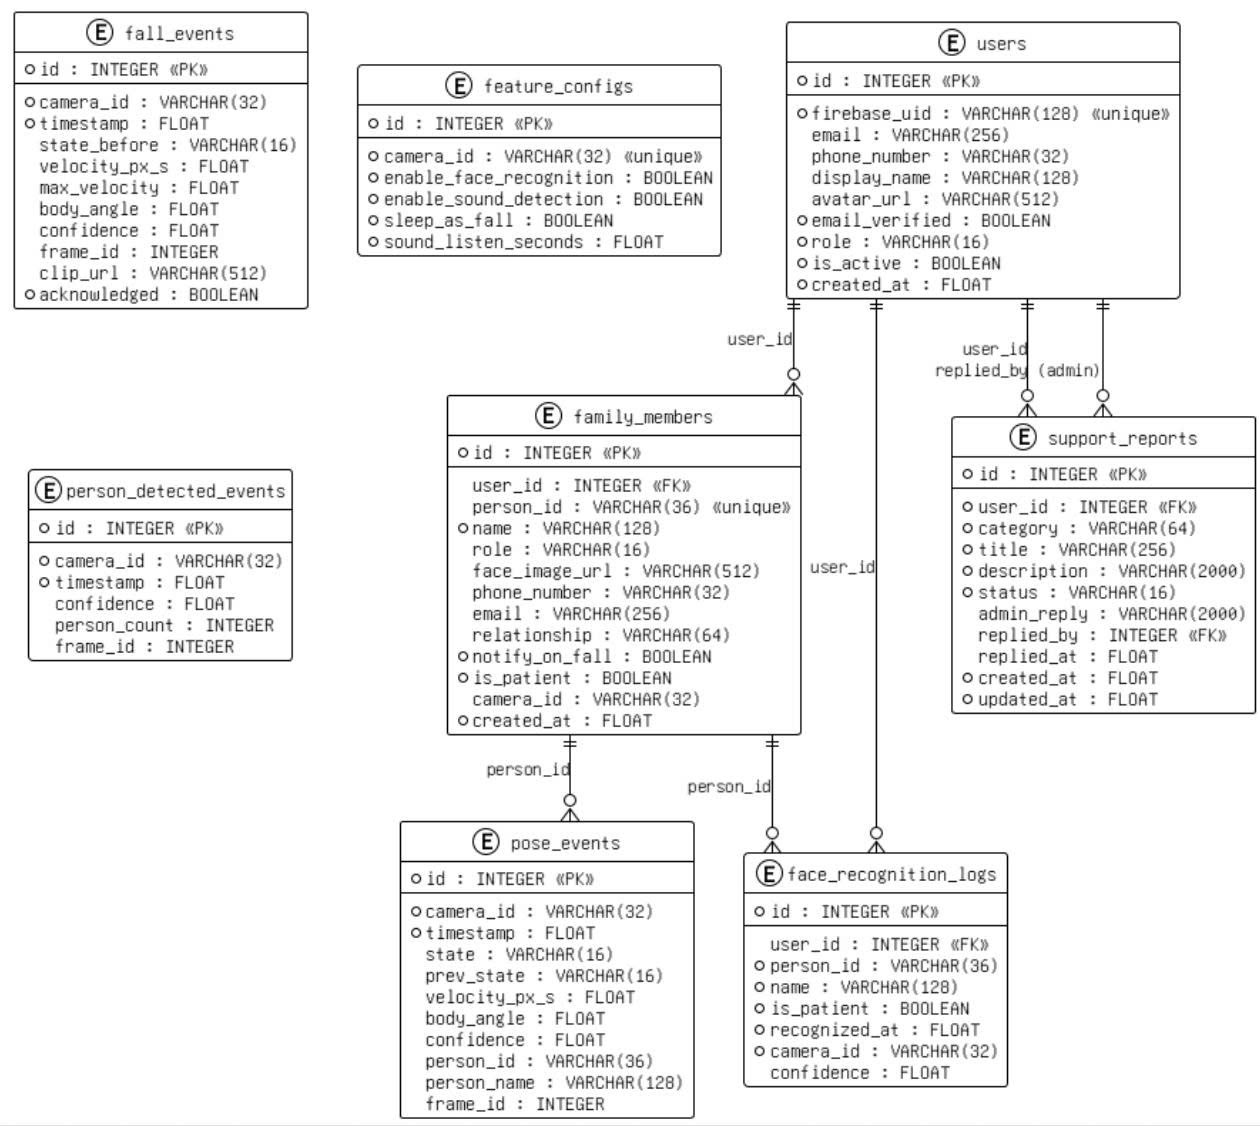
\includegraphics[width=1.0\textwidth]{figures/erd.jpg}
    \caption{Sơ đồ ERD}
    \label{fig:erd}
\end{figure}

\subsection*{Mô tả ERD}

Sơ đồ thực thể quan hệ (ERD) của hệ thống gồm tám bảng chính, được tổ chức xoay quanh bảng trung tâm \textit{users} và các bảng sự kiện phát sinh từ quá trình giám sát.

\subsubsection*{Các thực thể}

\textbf{users} là bảng trung tâm của hệ thống, lưu trữ thông tin tài khoản người dùng bao gồm định danh Firebase (\textit{firebase\_uid}), email, số điện thoại, ảnh đại diện, vai trò và trạng thái hoạt động. Trường \textit{firebase\_uid} được ràng buộc duy nhất để đảm bảo mỗi tài khoản Firebase chỉ tương ứng với một người dùng trong hệ thống.

\textbf{family\_members} lưu thông tin người thân được đăng ký bởi người dùng, bao gồm tên, mối quan hệ, số điện thoại, ảnh khuôn mặt và các tuỳ chọn như nhận thông báo té ngã (\textit{notify\_on\_fall}) và đánh dấu là bệnh nhân (\textit{is\_patient}). Trường \textit{person\_id} được dùng làm định danh duy nhất để liên kết với dữ liệu nhận diện khuôn mặt.

\textbf{fall\_events} ghi nhận các sự kiện té ngã được phát hiện từ camera, lưu thông tin như trạng thái trước khi té, vận tốc di chuyển, góc cơ thể, độ tin cậy, mã khung hình và đường dẫn video clip. Trường \textit{acknowledged} đánh dấu sự kiện đã được người dùng xác nhận hay chưa.

\textbf{pose\_events} lưu các sự kiện tư thế bất thường phát hiện trong quá trình giám sát, bao gồm trạng thái hiện tại, trạng thái trước đó, vận tốc, góc cơ thể và thông tin người được nhận diện thông qua \textit{person\_id} và \textit{person\_name}.

\textbf{face\_recognition\_logs} ghi lại lịch sử mỗi lần hệ thống nhận diện được khuôn mặt, bao gồm tên đối tượng, thời điểm nhận diện, độ tin cậy và camera thực hiện nhận diện. Trường \textit{is\_patient} phân biệt đối tượng là bệnh nhân hay người thân thông thường.

\textbf{support\_reports} lưu các báo cáo hỗ trợ do người dùng gửi lên, gồm danh mục, tiêu đề, nội dung mô tả và trạng thái xử lý. Bảng có hai khoá ngoại trỏ đến \textit{users}: \textit{user\_id} xác định người gửi báo cáo và \textit{replied\_by} xác định quản trị viên đã phản hồi.

\textbf{feature\_configs} lưu cấu hình tính năng theo từng camera, bao gồm các cờ bật/tắt nhận diện khuôn mặt, phát hiện âm thanh, chế độ coi trạng thái ngủ là té ngã và thời gian lắng nghe âm thanh. Trường \textit{camera\_id} được ràng buộc duy nhất, đảm bảo mỗi camera chỉ có một bộ cấu hình.

\textbf{person\_detected\_events} ghi nhận các sự kiện phát hiện người trong khung hình, lưu thông tin camera, thời điểm, số lượng người phát hiện và độ tin cậy. Bảng này phục vụ mục đích thống kê và phân tích hoạt động giám sát.

\subsubsection*{Quan hệ giữa các thực thể}

Bảng \textit{users} có quan hệ một-nhiều với \textit{family\_members}, \textit{face\_recognition\_logs} và \textit{support\_reports} thông qua khoá ngoại \textit{user\_id}, phản ánh việc mỗi người dùng có thể quản lý nhiều người thân, có nhiều lịch sử nhận diện và gửi nhiều báo cáo. Ngoài ra, \textit{users} còn có quan hệ một-nhiều với \textit{support\_reports} qua trường \textit{replied\_by}, thể hiện vai trò quản trị viên khi phản hồi báo cáo.

Bảng \textit{family\_members} có quan hệ một-nhiều với \textit{face\_recognition\_logs} và \textit{pose\_events} thông qua trường \textit{person\_id}, cho phép truy vết toàn bộ lịch sử nhận diện và các sự kiện tư thế gắn với từng người thân cụ thể.